\documentclass[12pt,AutoFakeBold]{article} 

\usepackage[数字信号处理]{XDULabreport}  % 载入 XDULabreport 模板文件,[]中填写科目名称,科目名称,默认为电子线路实验(I)
\problem{FIR 数字滤波器设计及结构}  % 请在此处填写问题内容
\labdate{2021年12月30日} % 实验日期
% 其他参数在宏包中进行更改,其中学院,班级,姓名,学号均在sty宏包内进行更改
% \usepackage{fourier}  % 这是 fourier 字体,更柔和 

\newfontfamily\digi{DigifaceWide Regular} % 将数码管字体引入

%% 如果你需要中文的一级标题编号,如“一、”、“二、”等,请把下面两行取消注释
% \RequirePackage{zhnumber} % change section number to chinese
% \titleformat{\section}{\Large\bfseries\rmfamily}{\zhnum{section}、}{0em}{}

% 文档开始
        
\begin{document}

\maketitle
\setcounter{tocdepth}{2}
\tableofcontents  % 生成目录

% 正文标题
\makeatletter
\begin{center}
    \LARGE \textbf{\textsf{\@problem}}
\end{center}
\makeatother

\section{实验目的}

设计计算机程序,根据滤波器的主要技术指标设计线性相位 FIR 数字低通、高通、带通和带阻滤波器;绘制滤波器的幅频特性和相频特性曲线,验证滤波器的设计结果是否达到设计指标要求;画出线性相位 FIR 数字滤波器的结构信号流图。

\section{实验原理}

\subsection{线性相位 FIR 数字滤波器}

FIR 数字滤波器是指滤波器的单位脉冲响应 $h(n)$ 是有限长序列。$N-1$ 阶 FIR 数字滤波器的系统函数 $H(z)$ 可表示为
%
\begin{equation}
H(z)=\sum_{n=0}^{N-1}h(n)z^{-n}
\end{equation}
%
$H(z)$ 是 $z^{-1}$ 的 $N-1$ 阶多项式,在 $z$ 平面上有 $N-1$ 个零点,而它的 $N-1$ 个极点均位于 $z$ 平面的原点 $z=0$。

FIR 数字滤波器的频率响应
%
\begin{equation}
H(e^{j\omega})=\sum_{n=0}^{N-1}h(n)e^{-j\omega n}
\end{equation}
%
一般可将 $H(e^{j\omega})$ 表示成如下形式:
%
\begin{equation}
H(e^{j\omega})=H(\omega)e^{j\theta(\omega)}
\end{equation}
%
式中,$H(\omega)$ 是一个可取正值也可取负值的实函数,称为幅度特性函数,它与 $H(e^{j\omega})=|H(e^{j\omega})|e^{j\phi(\omega)}$ 中的幅频响应函数 $|H(e^{j\omega})|$ 是不同的;$\theta(\omega)$ 也与相频响应函数 $\phi(\omega)$ 不同,称为相位特性函数。

\subsection{FIR 数字滤波器的窗函数设计法}

\subsubsection{窗函数设计法的基本原理}

设 $H_d(e^{j\omega})$ 是希望逼近滤波器的频率响应函数,则由其 IDTFT 可得出滤波器的单位脉冲响应
%
\begin{equation}
h_d(n)=\frac{1}{2\pi}\int_{-\pi}^{\pi}H_d(e^{j\omega})e^{j\omega n}\mathrm{d}\omega
\end{equation}
%
窗函数设计法的基本思想是用所设计的 FIR 滤波器频率响应特性去逼近希望滤波器的频率响应特性。为了设计方便,通常选择 $H_d(e^{j\omega})$ 为具有分段常数特性的理想滤波器,因此其 $h_d(n)$ 是无限长非因果序列。为了能用 FIR 滤波器来近似理想滤波器,需要将理想滤波器的无限长单位脉冲响应 $h_d(n)$,截取为长度为 $N$ 的因果序列,并用合适的窗函数进行加权,结果作为 FIR 数字滤波器的单位脉冲响应 $h(n)(0\le n\le N-1)$

这种在 $0\le n\le N-1$ 范围内截取 $h_d(n)$ 的有限长序列作为所设计 FIR 数字滤波器的单位脉冲响应 $h(n)$,是基于最小均方误差准则。理想滤波器的频率响应 $H_d(e^{j\omega})$ 与设计滤波器的频率响应 $H(e^{j\omega})$ 的均方误差定义为
%
\begin{equation}
\epsilon^2=\frac{1}{2\pi}\int_{-\pi}^{\pi}|H_d(e^{j\omega})-H(e^{j\omega})|^2\mathrm{d}\omega
\end{equation}
%
根据帕塞瓦尔定理,$\epsilon^2$ 可表示为
%
\begin{equation}
\begin{aligned}
\epsilon^2 &= \sum_{n=-\infty}^{\infty}|h_d(n)-h(n)|^2 \\
           &= \sum_{n=-\infty}^{-1}|h_d(n)|^2\sum_{n=0}^{N-1}|h_d(n)-h(n)|^2+\sum_{n=N}^{\infty}|h_d(n)|^2
\end{aligned}
\end{equation}
%
式中,第一项和第三项与设计的滤波器参数无关,为使 $\epsilon^2$ 最小,应使式中第二项达到最小,于是可取
%
\begin{equation} \label{eq:h(n)}
h(n)=h_d(n),\quad 0\le n\le N-1
\end{equation}
%
所以用上述方法所设计的 FIR 数字滤波器是在均方误差最小下的最佳滤波器。

(\ref{eq:h(n)}) 式表明,所设计的 FIR 数字滤波器单位脉冲响应 $h(n)(0\le n\le N-1)$ 是理想滤波器的单位脉冲响应 $h_d(n)$ 加矩形窗函数 $R_N(n)$ 截断得到的,即
%
\begin{equation}
h(n)=h_d(n)R_N(n)
\end{equation}
%
为了改善所设计的 FIR 数字滤波器的整体性能,对 $h_d(n)$ 截断的窗函数还可以采用其他的函数形式,记为 $w(n)$。这样,$h(n)$ 一般地表示为
%
\begin{equation}
h(n)=h_d(n)w(n)
\end{equation}
%
所以我们把这种设计方法称为窗函数设计法。

一般来说,窗函数应满足如下两个要求:
\begin{enumerate}[(1)]
\item 主瓣宽度要窄,以获得较窄的滤波器过渡带宽。
\item 窗函数的时域波形平滑,与主瓣的幅度相比,旁瓣应尽可能小,以减小滤波器的通带衰减,增大阻带衰减,提高滤波器的性能。
\end{enumerate}

为了描述方便并便于比较,需要定义表征窗函数特性的主要参数,简述如下。

旁瓣电平 $\alpha_e$:窗函数幅度特性绝对值 $|W(\omega)|$ 的最大旁瓣的最大值相对于主瓣的最大值的比值 (dB)。
过渡带宽度 $\Delta B$:用窗函数所设计的 FIR 数字滤波器的过渡带宽度 (rad)。
阻带最小衰减 $\alpha_s$: 用窗函数所设计的 FIR 数字滤波器的阻带最小衰减 (dB)。

\subsubsection{窗函数法设计 FIR 数字滤波器的步骤}

\begin{enumerate}[(1)]
\item 根据所需设计的数字滤波器类型 (低通、高通、带通、带阻),确定线性相位数字滤波器类型 (I 型、II 型、III 型、IV 型)。
\item 选择合适的窗函数 $w(n)$。

根据滤波器阻带衰减 $\alpha_s$,选择窗函数 $w(n)$ 的种类,然后根据滤波器过渡带宽度确定所选窗函数的长度 $N$,并可根据线性相位数字滤波器类型,对 $N$ 向大修正。应当说明,用窗函数法设计的 FIR 数字滤波器的通带波纹幅度近似等于阻带波纹幅度。一般要求滤波器的阻带最小衰减达到 40dB($\delta_s\le0.01$) 以上,则通带最大衰减就小于 0.1dB($\delta_p\le0.01$)。所以用窗函数法设计 FIR 滤波器时,通常只考虑阻带最小衰减就可以了。
\item 确定理想数字滤波器的频率响应函数 $H_d(e^{j\omega})=H_d(\omega)e^{j\theta_d(\omega)}$,其中 $H_d(\omega)$ 是幅度特性函数, $\theta_d(\omega)$ 是相位特性函数.

对 I 型和 II 型严格线性相位 FIR 数字滤波器,$θ_d(\omega)=-\omega(N-1)/2$;对 III 型和 IV 型广义线性相位 FIR 数字滤波器,$θ_d(\omega)=-\pi/2-\omega(N-1)/2$。一般取滤波器截止频率 $\omega_c=(\omega_p+\omega_s)/2$,其中 $\omega_p$ 和 $\omega_s$ 分别为通带边界频率和阻带边界频率。
\item 计算理想滤波器的单位脉冲响应 $h_d(n)$,即
%
\begin{equation}
h_d(n)=\frac{1}{2\pi}\int_{-\pi}^{\pi}H_d(e^{j\omega})e^{j\omega n}\mathrm{d}\omega
\end{equation}
%
\item 加窗得到设计结果 $h(n)$,即:
%
\begin{equation}
h(n)=h_d(n)w(n)
\end{equation}
%
\end{enumerate}

\section{实验过程}

所有设计均为第一类线性相位数字滤波器。

Matlab 提供了窗函数法设计 FIR 数字滤波器的函数 fir1,格式为:\lstinline[language=Matlab]|h=fir1(N,Wc,'ftype',window)|,其中 h 是数字滤波器的单位脉冲响应,长度为 $N+1$。Wc 是对 $\pi$ 归一化的 6dB 数字截止频率,$0\le W_c\le1$。

ftype 是滤波器类型,当 ftype 缺省,并且 Wc 是标量时,设计低通滤波器;当 ftype 缺省,并且 Wc 是标量时,设计低通滤波器;当 ftype 缺省,并且 Wc=[Wcl,Wcu] 时,设计带通滤波器,其 -6dB 通带为 Wcl$\le\omega\le$Wcu;当 ftype=high 时,设计高通滤波器;当 ftype=stop,并且 Wc=[Wcl,Wcu] 时,设计带阻滤波器。在设计高通和带阻滤波器时,$N$ 只能取偶数;如果将 $N$ 设置为奇数,fir1 会自动对 $N$ 加 1。

window 是窗函数的类型,当 window 缺省时,采用汉明窗函数;当 window=bartlett($N$+1) 时,采用三角窗;当 window=hanning($N$+1) 时,采用汉宁窗;当 window=blackman($N$+1) 时,采用布莱克曼窗;当 window=kaiaer($N$+1,beta) 时,采用 $\beta=$beta 的凯塞窗函数。


\subsection{FIR 数字低通滤波器}

假设指标要求为:通带截止频率 $\omega_p=0.2\pi\mathrm{rad}$,阻带截止频率 $\omega_p=0.5\pi\mathrm{rad}$,通带最大衰减 $\alpha_p=1\mathrm{dB}$,阻带最小衰减 $\alpha_s=40\mathrm{dB}$。

采用凯塞窗函数设计,凯塞窗函数的调整参数
%
\begin{equation*}
\beta=0.5842(\alpha_s-21)^{0.4}+0.07886(\alpha_s-21)=3.3953
\end{equation*}
%
滤波器的阶数
%
\begin{equation*}
N-1=\frac{\alpha_s-7.95}{2.285\Delta B}=\frac{40-7.95}{2.285\times0.3\pi}=14.8823
\end{equation*}
%
取满足要求的最小整数 $N-1=15$,由于 I 型线性相位数字滤波器阶数必须为偶数,$N$ 为奇数,取 $N=17$。

理想低通滤波器的 6dB 截止频率 $\omega=(\omega_s+\omega_p)/2=0.35\pi\mathrm{rad}$。FIR 数字低通滤波器单位脉冲响应如图 \ref{fig:LP1} 所示。频率响应曲线如图 \ref{fig:LP2} 所示。$\omega=0.2$ 时幅度为 0dB,$\omega=0.5$ 时幅度为 -47.7dB,通带满足指标要求,阻带满足指标要求,过渡带比指标要求的窄。(查看幅度修改代码 \lstinline[language=Matlab]|[H,W] = freqz(h,1,512);| 中的参数 512 为 1000,并使用 Matlab 中图像的数据游标功能)

\begin{figure}[htbp]
	\centering
	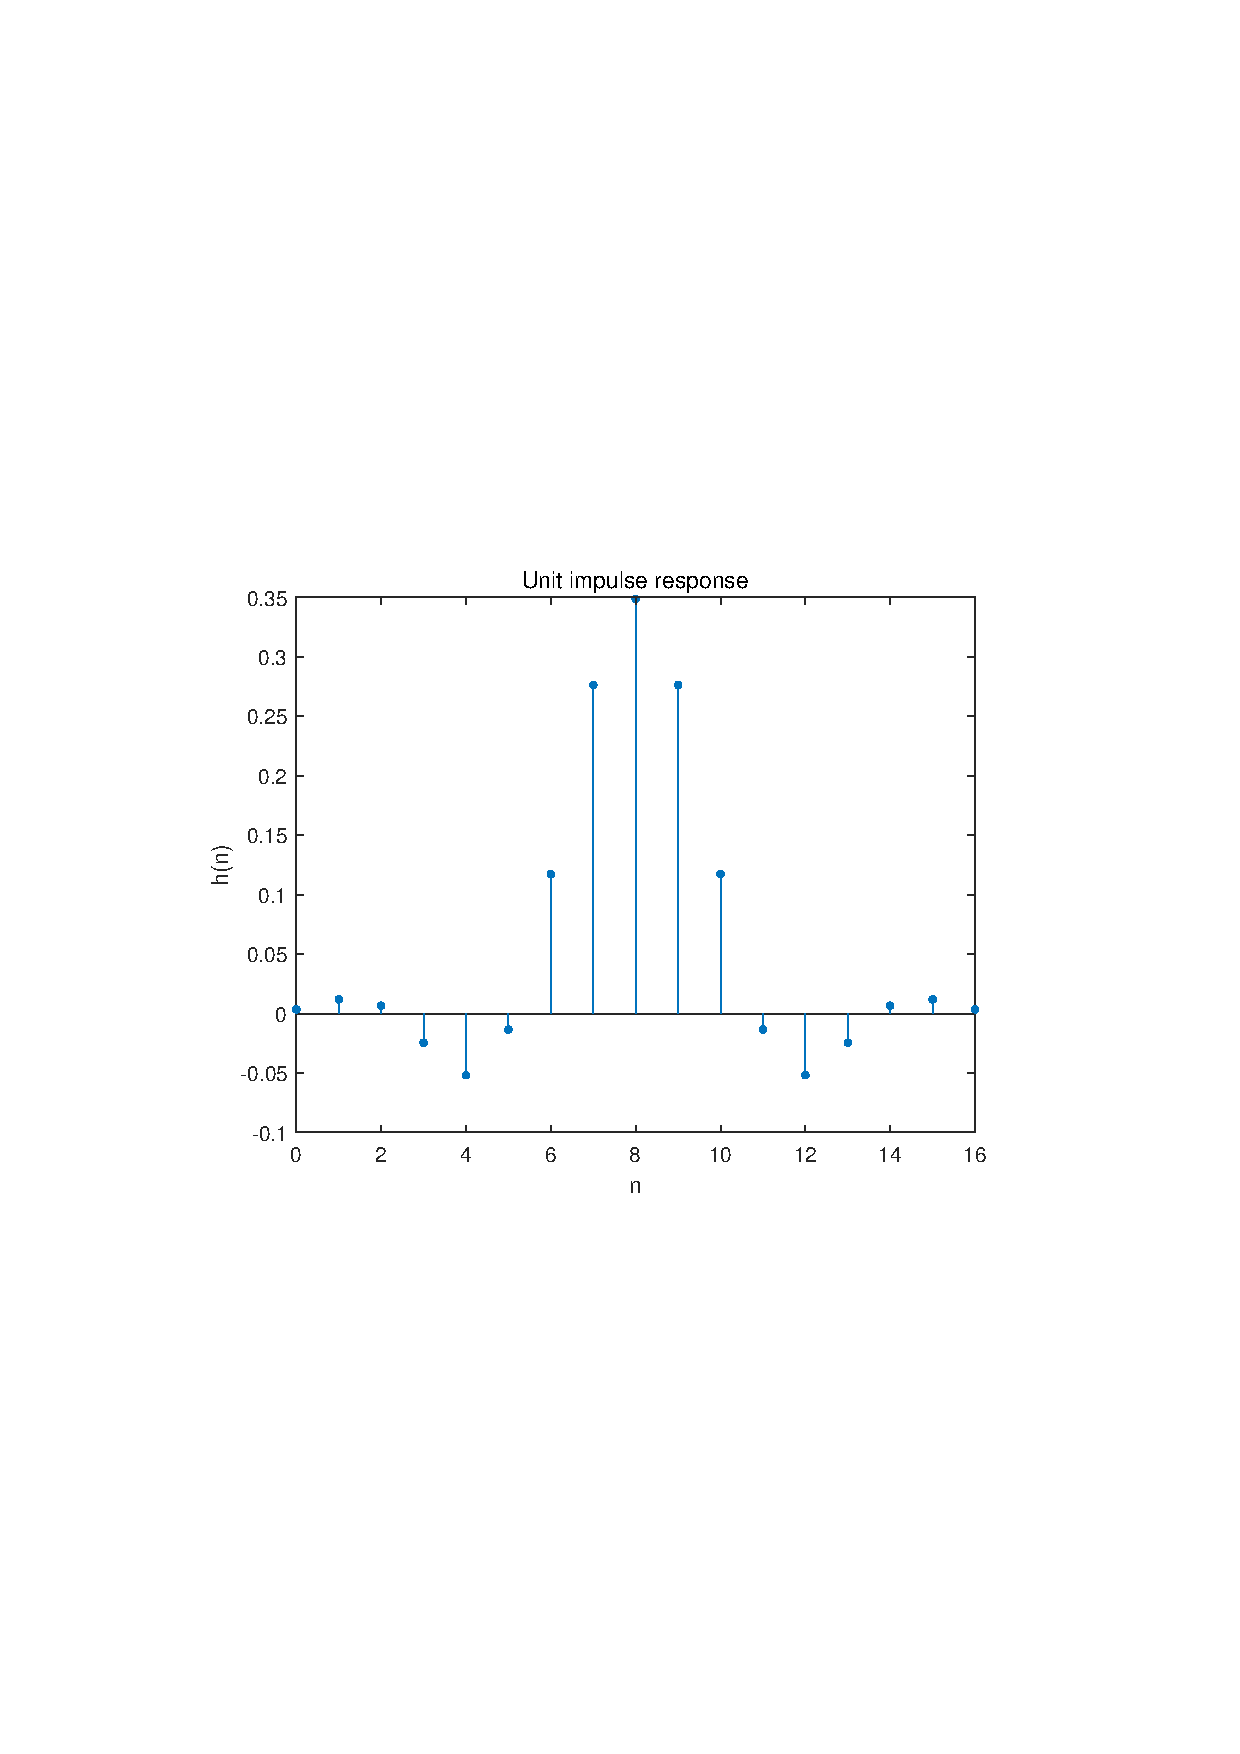
\includegraphics[width=0.5\textwidth]{figure/LP1.pdf}
	\caption{FIR 数字低通滤波器单位脉冲响应} \label{fig:LP1}
\end{figure}

\begin{figure}[htbp]
	\centering
	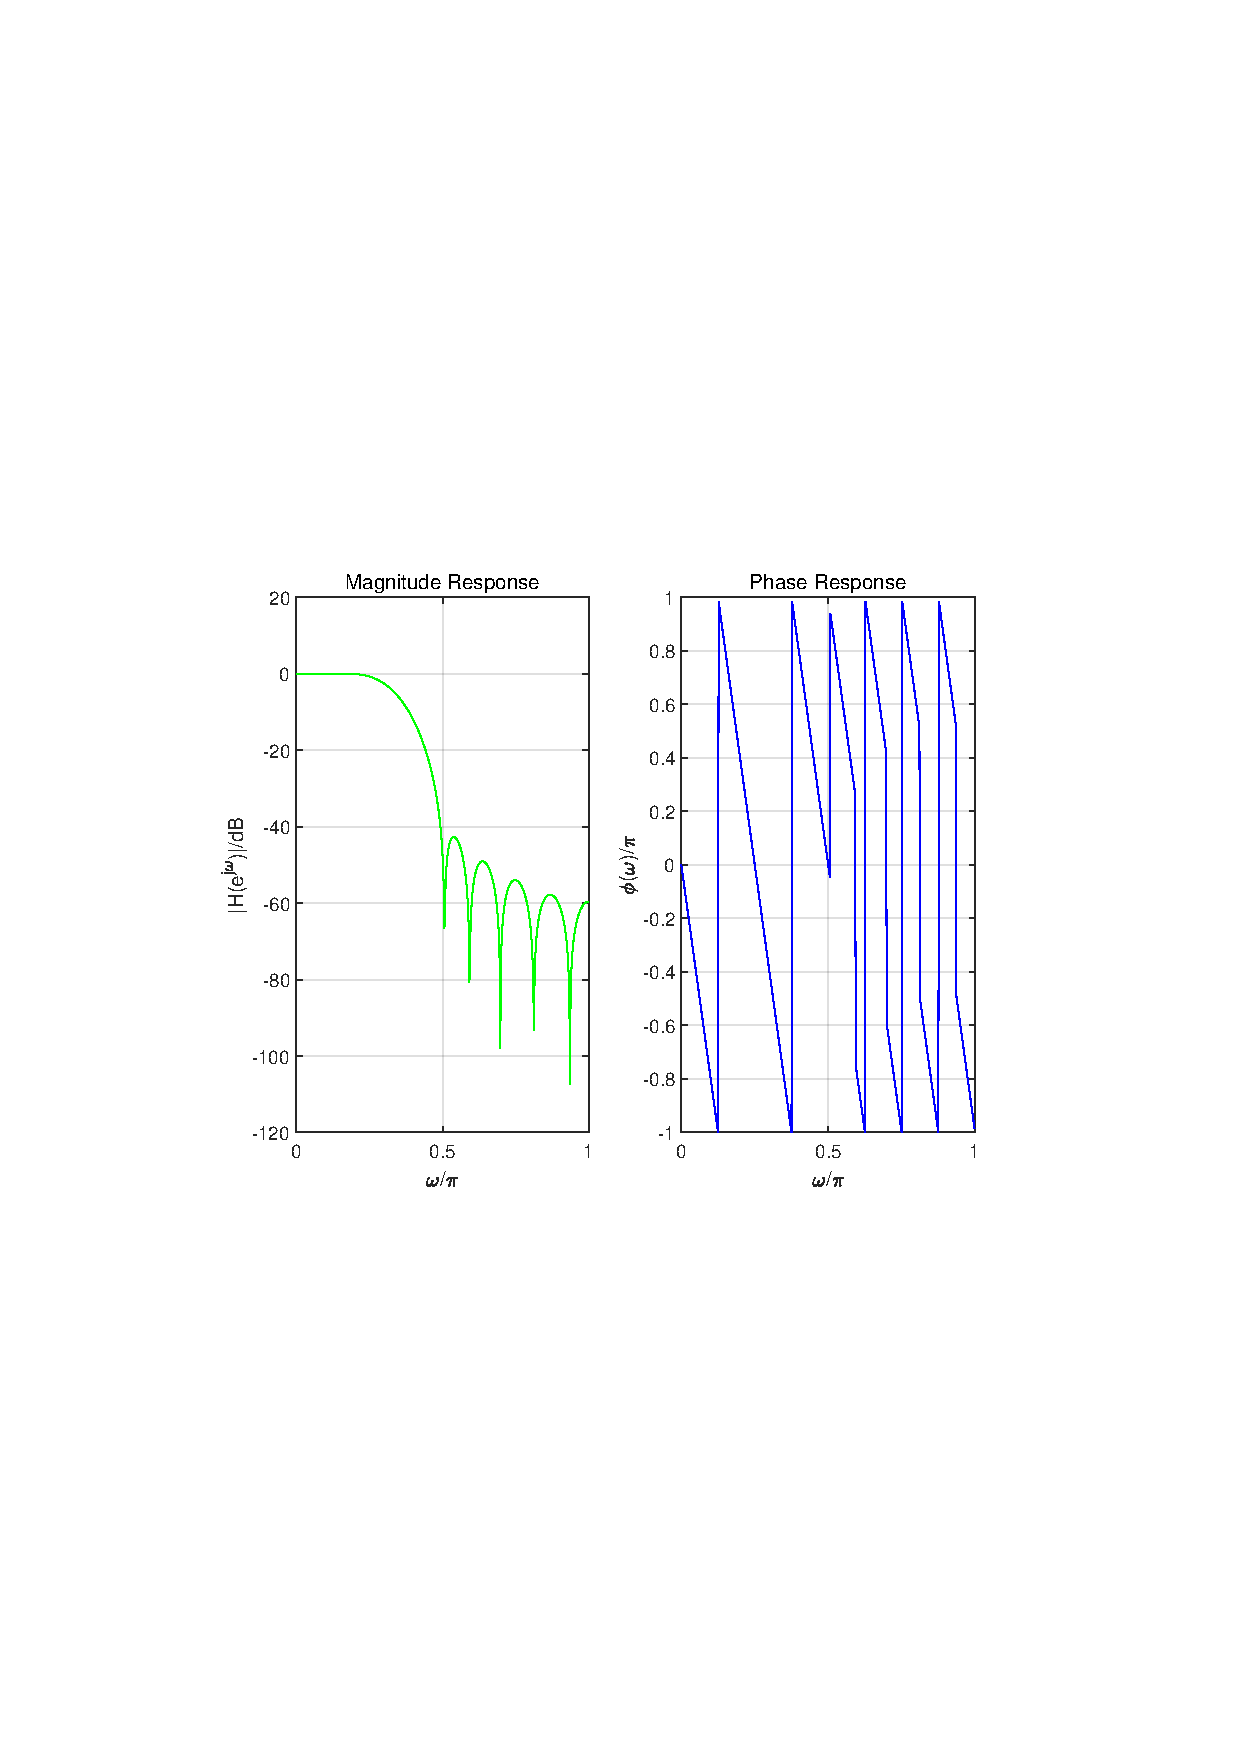
\includegraphics[width=0.7\textwidth]{figure/LP2.pdf}
	\caption{FIR 数字低通滤波器单位频率响应曲线} \label{fig:LP2}
\end{figure}

\subsection{FIR 数字高通滤波器}

假设指标要求为:通带截止频率 $\omega_p=0.5\pi\mathrm{rad}$,阻带截止频率 $\omega_p=0.2\pi\mathrm{rad}$,通带最大衰减 $\alpha_p=1\mathrm{dB}$,阻带最小衰减 $\alpha_s=40\mathrm{dB}$。

采用汉宁窗函数设计,要求过渡带宽度 $\Delta B=\frac{6.2\pi}{N}\le 0.3\pi$,解得 $N\ge20.7$。I 型滤波器的 N 必须取奇数,取 $N=21$,汉宁函数为
%
\begin{equation*}
w(n)=\begin{cases}
0.5\left[ 1 - \cos\left(\frac{\pi n}{10}\right) \right], & 0\le n\le 20 \\
0, & others
\end{cases}
\end{equation*}
%

理想高通滤波器的 6dB 截止频率 $\omega=(\omega_s+\omega_p)/2=0.35\pi\mathrm{rad}$。FIR 数字高通滤波器单位脉冲响应如图 \ref{fig:HP1} 所示。频率响应曲线如图 \ref{fig:HP2} 所示。$\omega=0.2$ 时幅度为 -60.9dB,$\omega=0.5$ 时幅度为 0dB,通带满足指标要求,阻带满足指标要求,过渡带比指标要求的窄。

\begin{figure}[htbp]
	\centering
	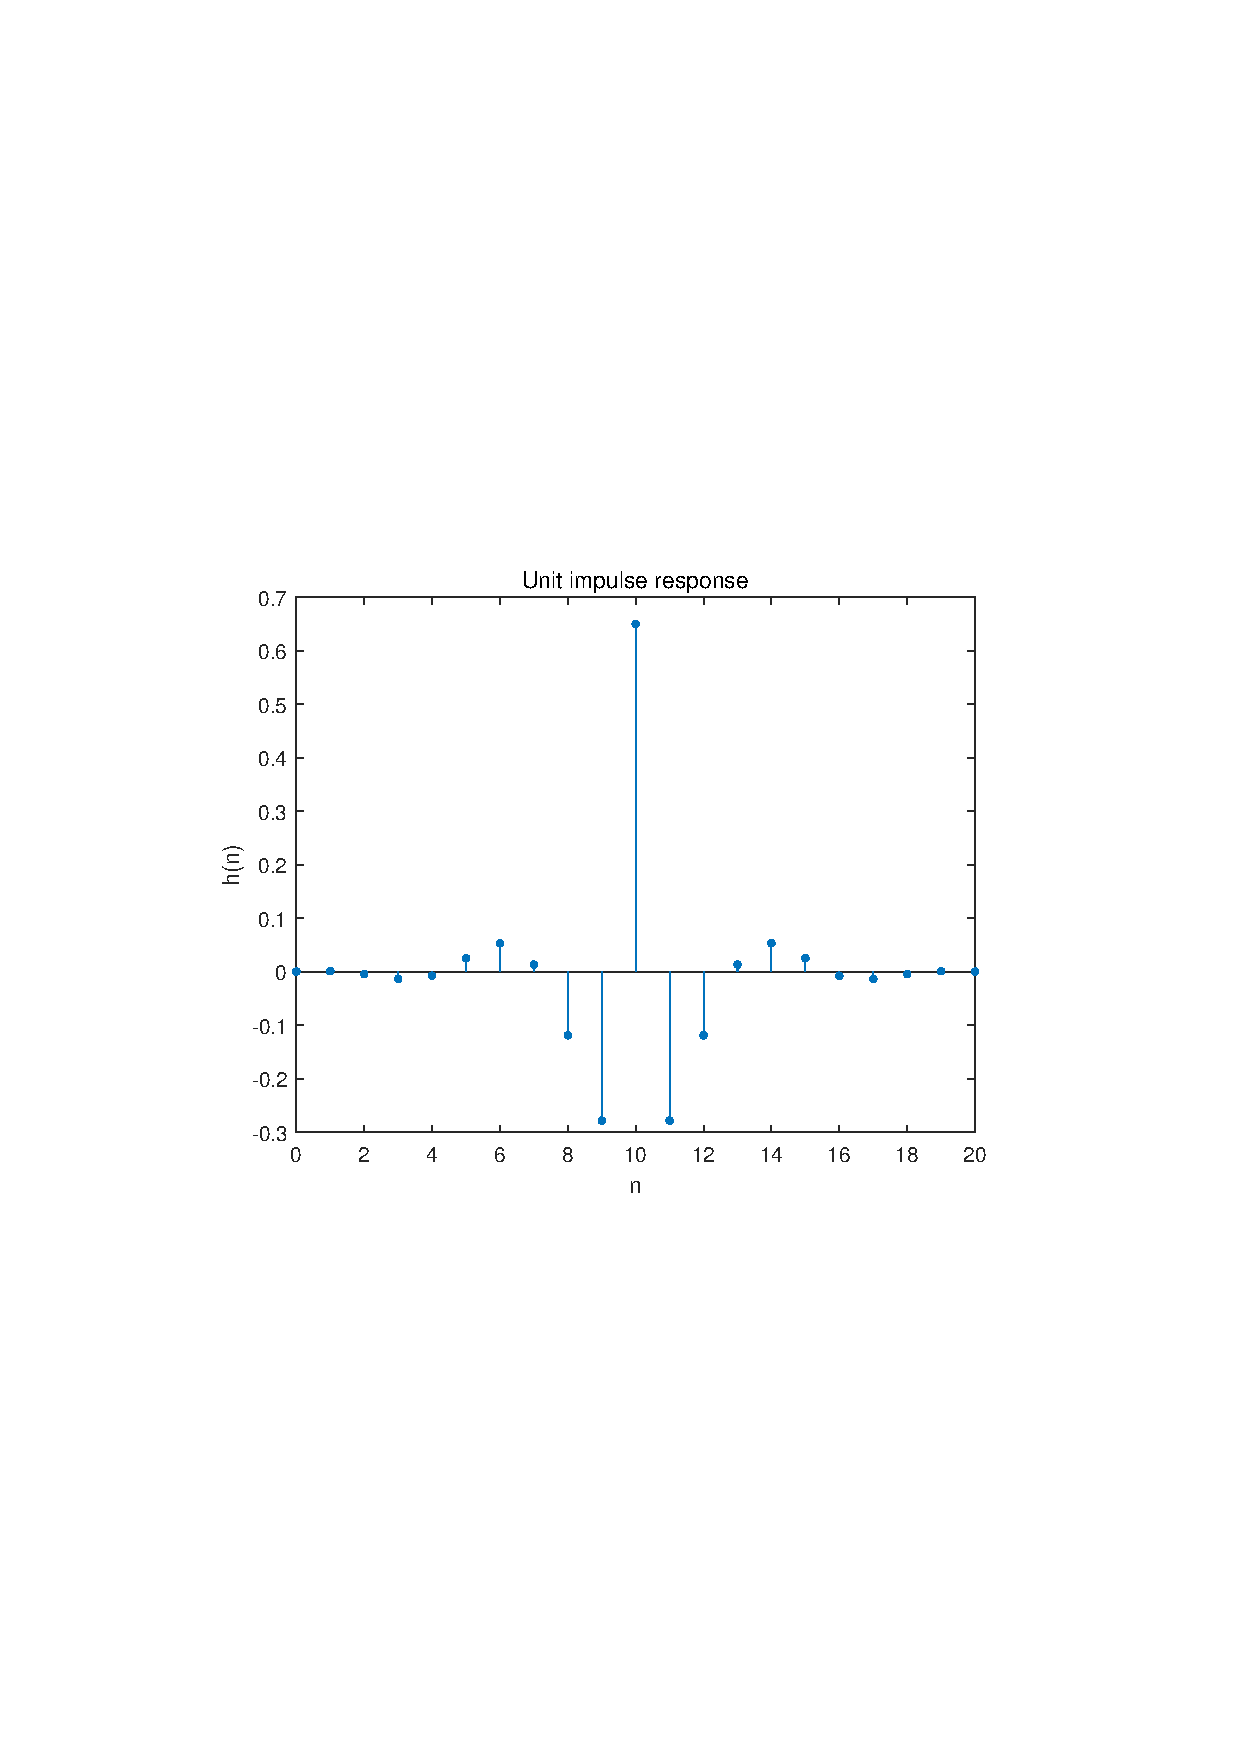
\includegraphics[width=0.5\textwidth]{figure/HP1.pdf}
	\caption{FIR 数字高通滤波器单位脉冲响应} \label{fig:HP1}
\end{figure}

\begin{figure}[htbp]
	\centering
	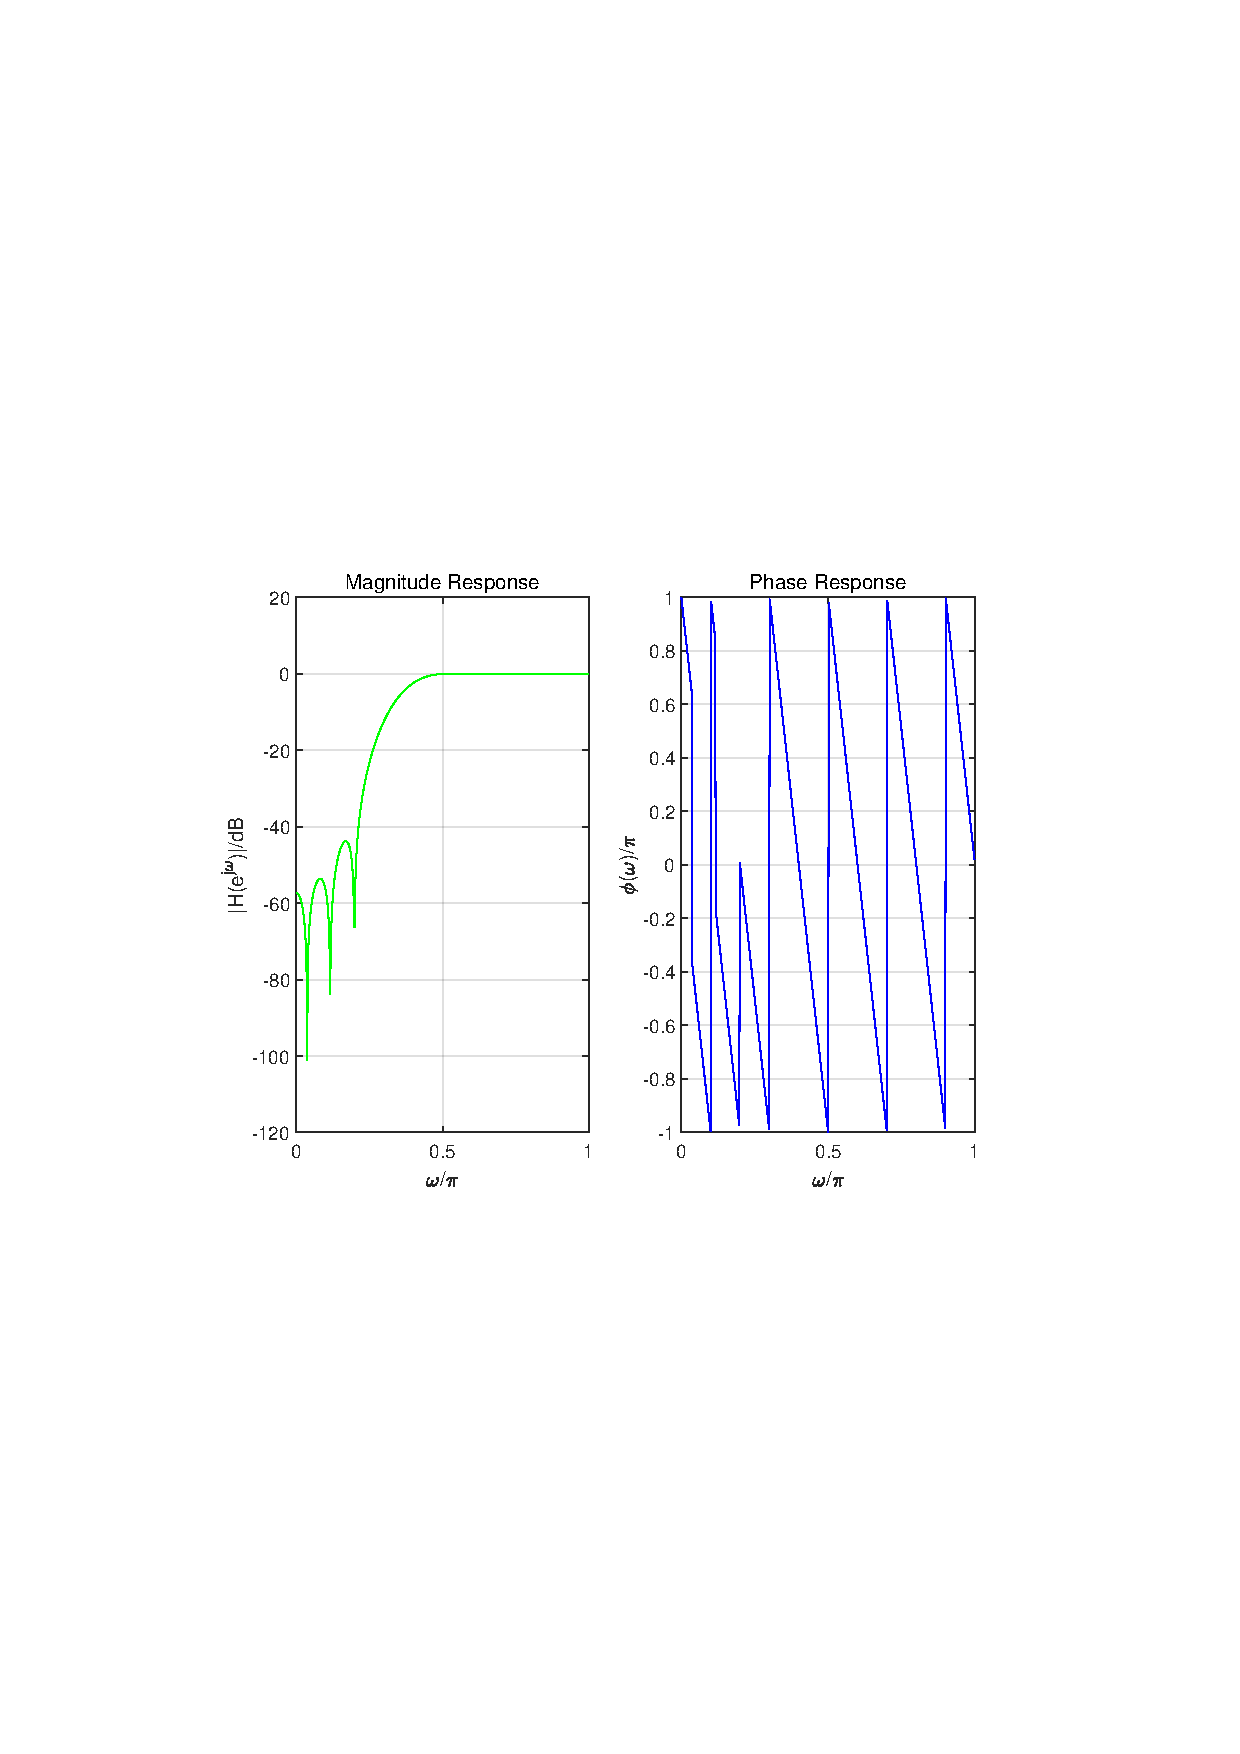
\includegraphics[width=0.7\textwidth]{figure/HP2.pdf}
	\caption{FIR 数字高通滤波器单位频率响应曲线} \label{fig:HP2}
\end{figure}

\subsection{FIR 数字带通滤波器}

假设指标要求为:通带截止频率 $\omega_p=[0.4\pi,0.6\pi]\mathrm{rad}$,阻带截止频率 $\omega_p=[0.2\pi,0.8\pi]\mathrm{rad}$,通带最大衰减 $\alpha_p=1\mathrm{dB}$,阻带最小衰减 $\alpha_s=40\mathrm{dB}$。

\begin{figure}[htbp]
	\centering
	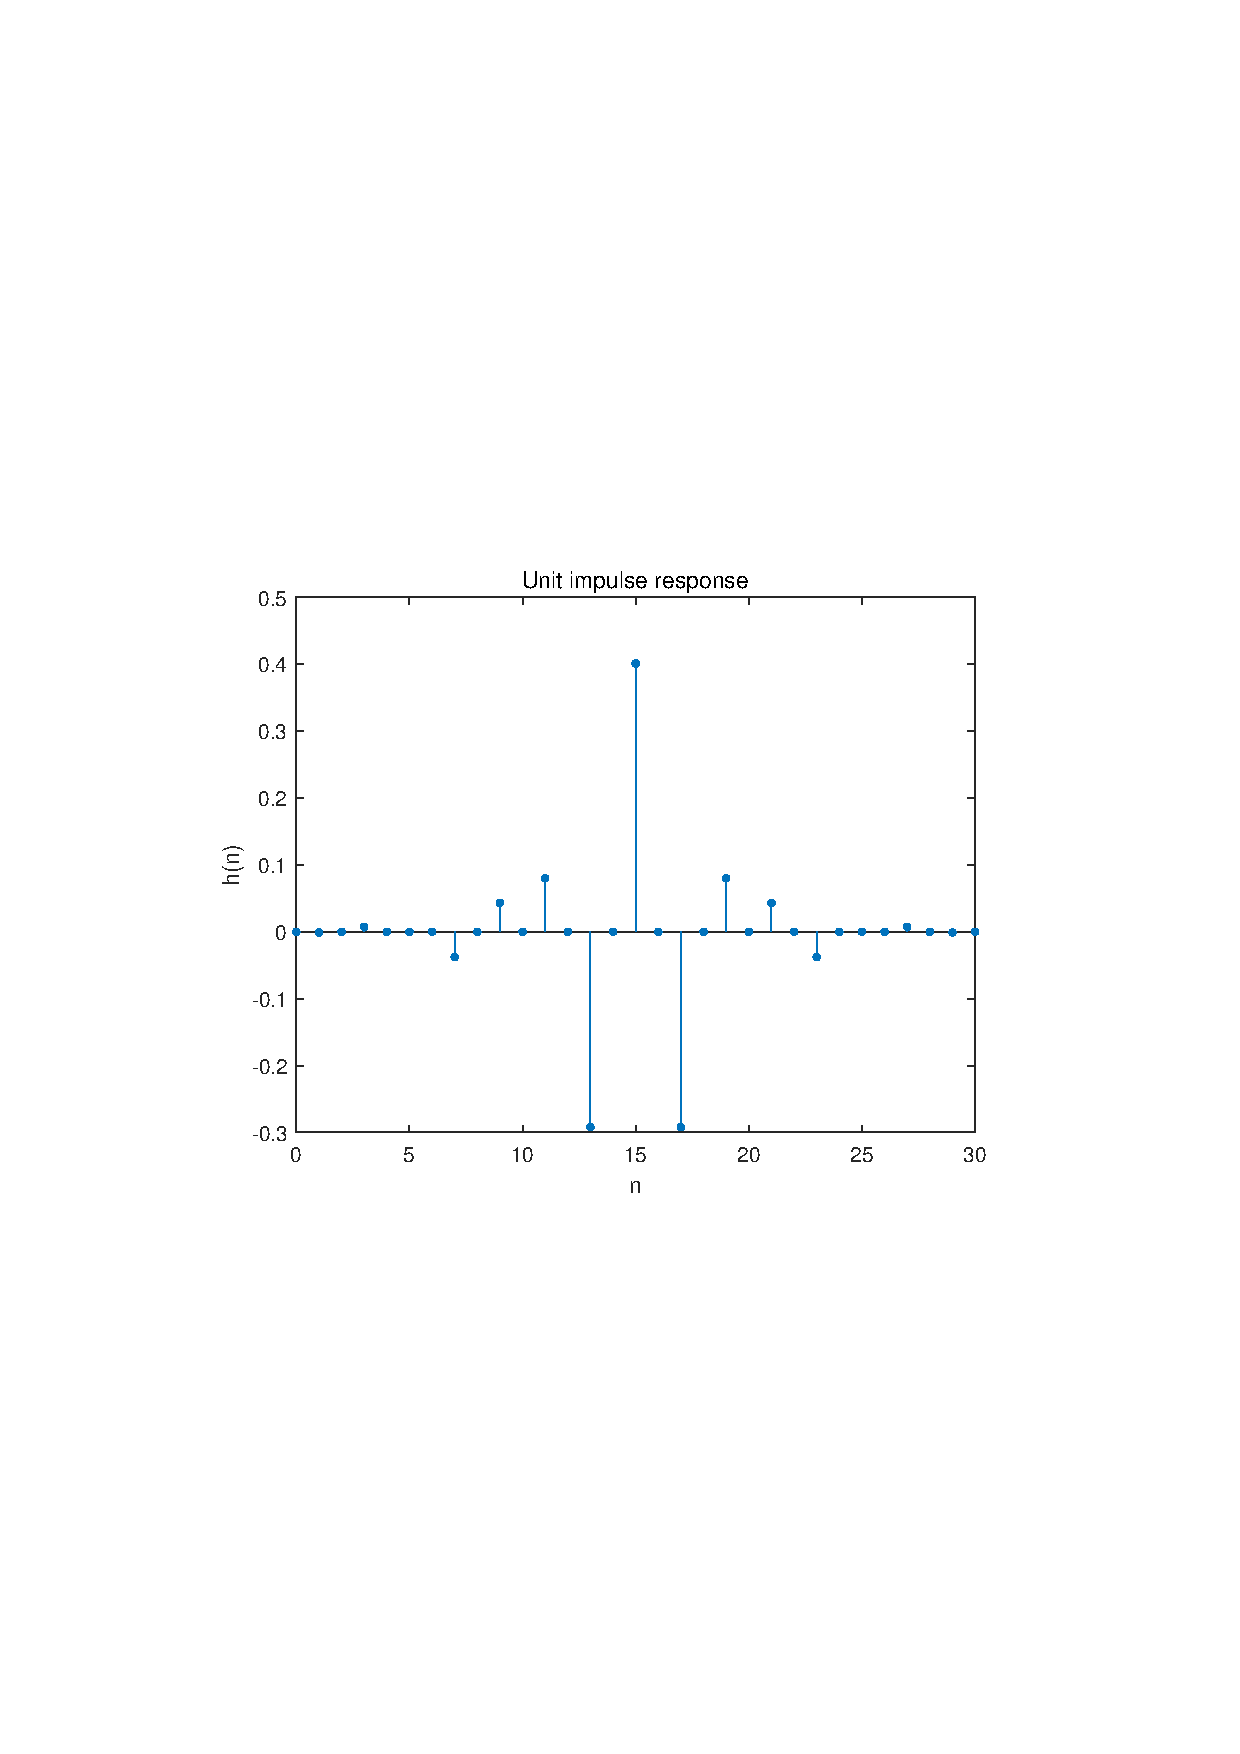
\includegraphics[width=0.5\textwidth]{figure/BP1.pdf}
	\caption{FIR 数字带通滤波器单位脉冲响应} \label{fig:BP1}
\end{figure}

采用汉宁窗函数设计,要求过渡带宽度 $\Delta B=\frac{6.2\pi}{N}\le 0.2\pi$,解得 $N\ge31$。取 $N=31$,汉宁函数为
%
\begin{equation*}
w(n)=\begin{cases}
0.5\left[ 1 - \cos\left(\frac{\pi n}{15}\right) \right], & 0\le n\le 30 \\
0, & others
\end{cases}
\end{equation*}
%

理想带通滤波器的 6dB 截止频率 $\omega=(\omega_s+\omega_p)/2=[0.3\pi,0.7\pi]\mathrm{rad}$。FIR 数字带通滤波器单位脉冲响应如图 \ref{fig:BP1} 所示。频率响应曲线如图 \ref{fig:BP2} 所示。$\omega=0.2$ 时幅度为 -48.2dB,$\omega=0.8$ 时幅度为 -48.2dB,$\omega=0.4$ 时幅度为 0dB,$\omega=0.6$ 时幅度为 0dB,通带满足指标要求,阻带满足指标要求,过渡带比指标要求的窄。


\begin{figure}[htbp]
	\centering
	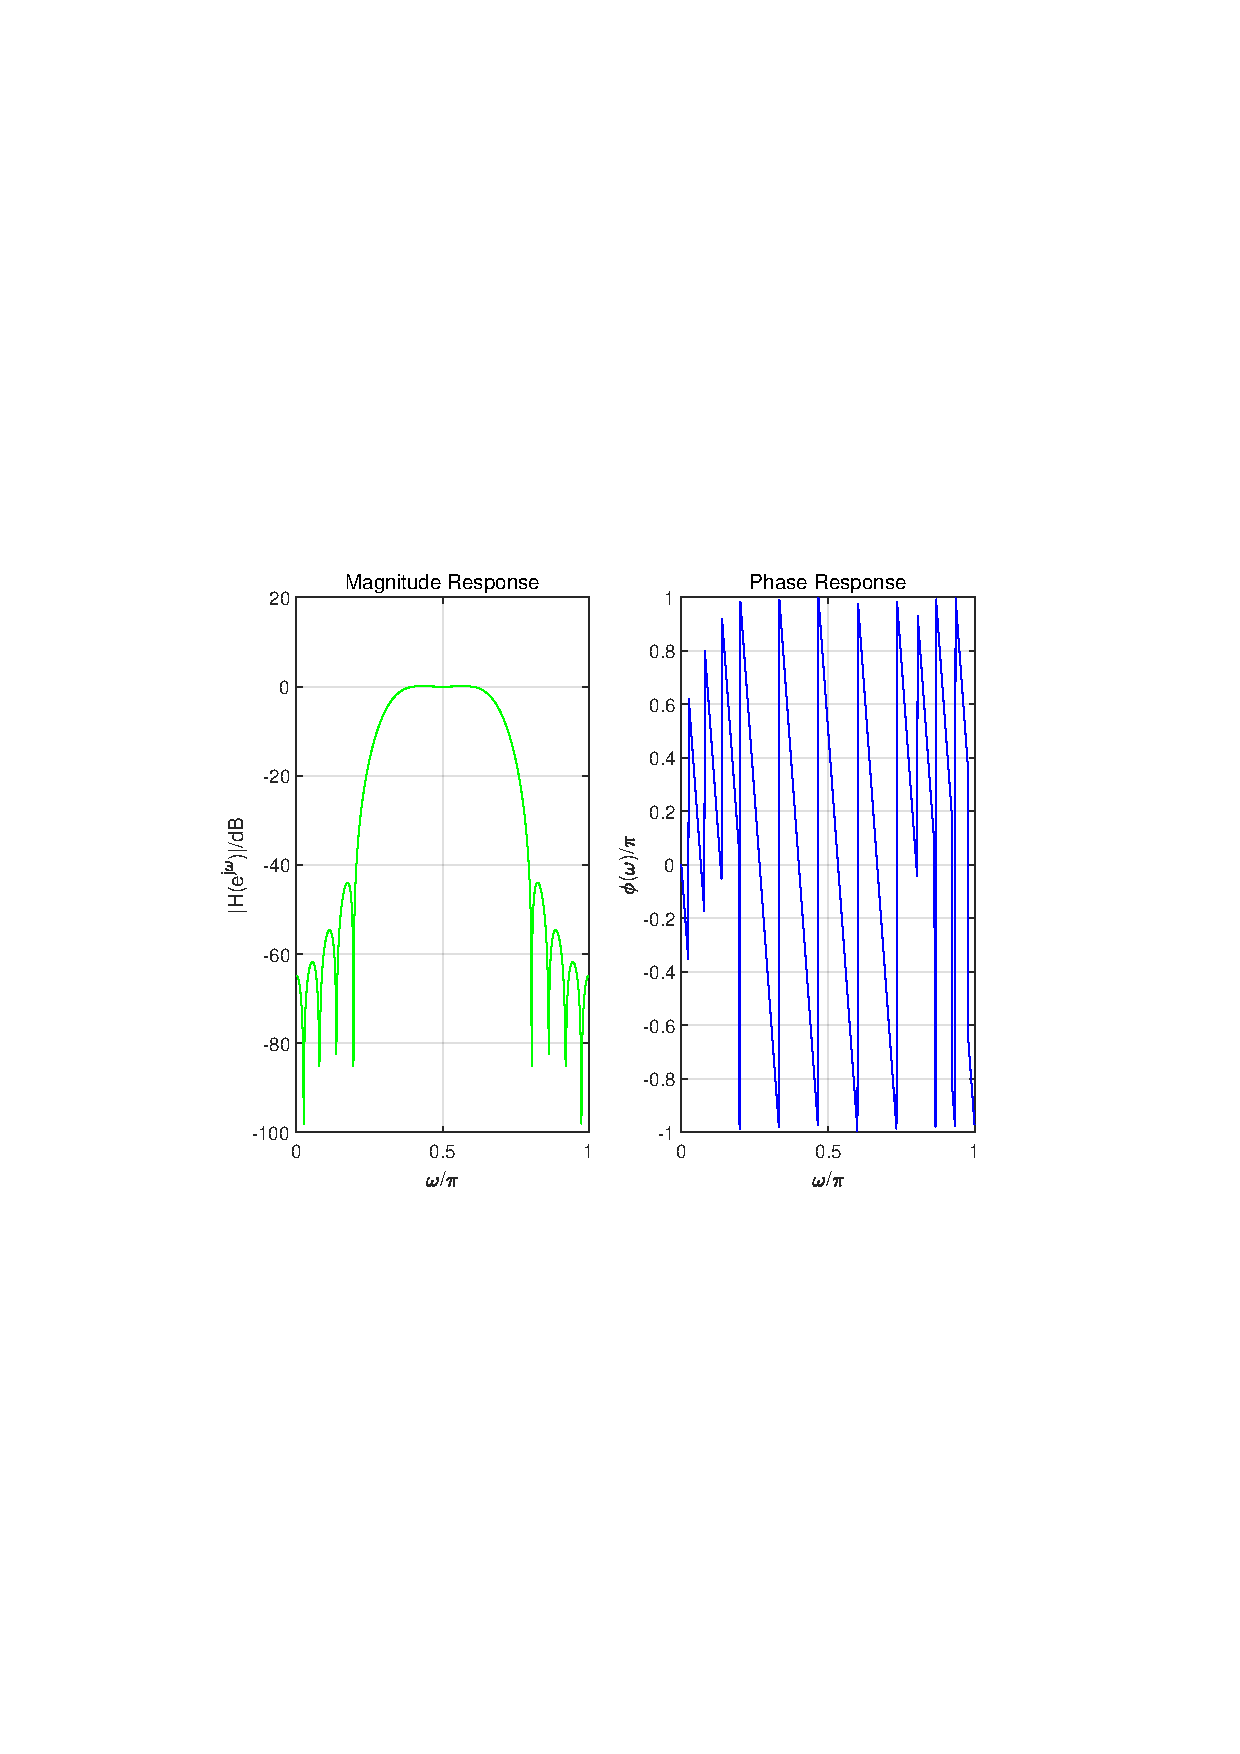
\includegraphics[width=0.7\textwidth]{figure/BP2.pdf}
	\caption{FIR 数字带通滤波器单位频率响应曲线} \label{fig:BP2}
\end{figure}

\subsection{FIR 数字带阻滤波器}

假设指标要求为:通带截止频率 $\omega_p=[0.2\pi,0.8\pi]\mathrm{rad}$,阻带截止频率 $\omega_p=[0.4\pi,0.6\pi]\mathrm{rad}$,通带最大衰减 $\alpha_p=1\mathrm{dB}$,阻带最小衰减 $\alpha_s=40\mathrm{dB}$。

\begin{figure}[htbp]
	\centering
	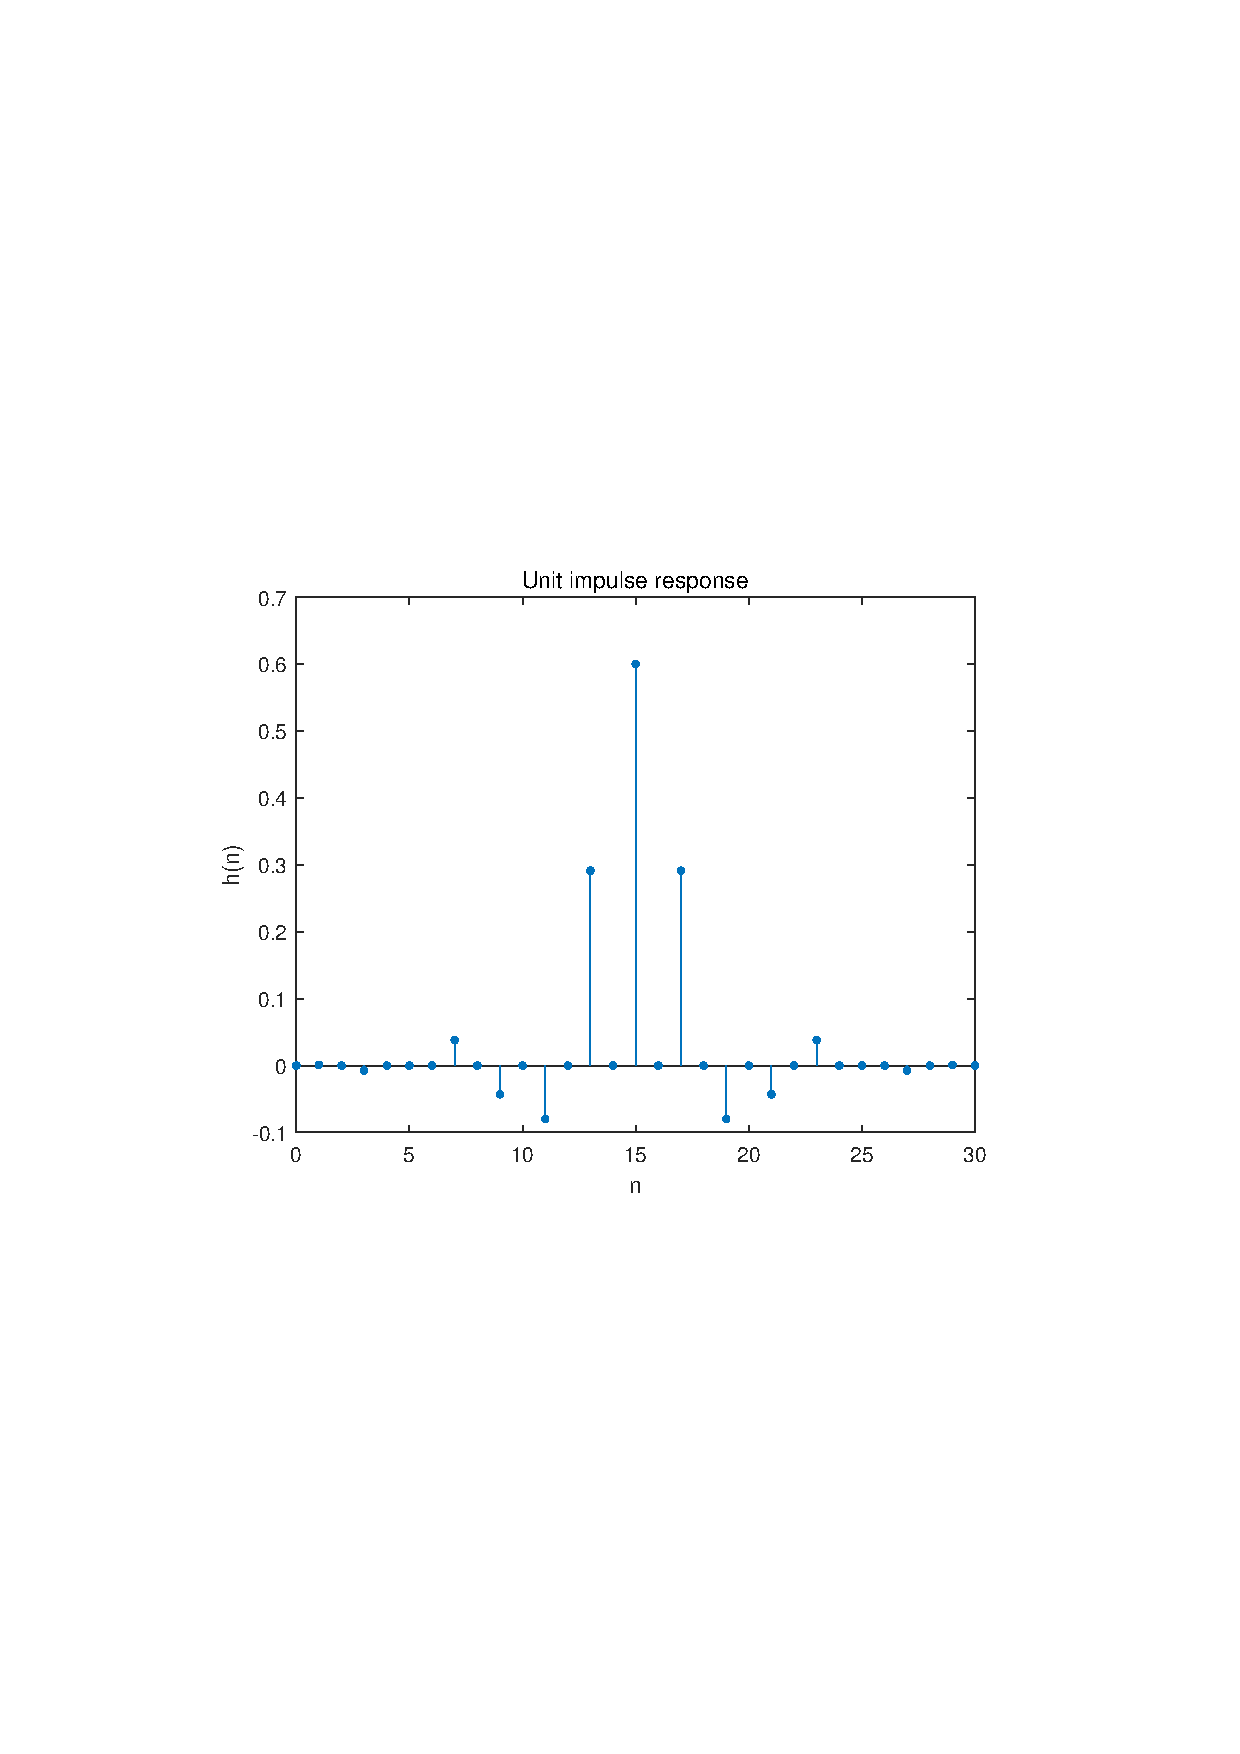
\includegraphics[width=0.5\textwidth]{figure/BS1.pdf}
	\caption{FIR 数字带阻滤波器单位脉冲响应} \label{fig:BS1}
\end{figure}

采用汉宁窗函数设计,要求过渡带宽度 $\Delta B=\frac{6.2\pi}{N}\le 0.2\pi$,解得 $N\ge31$。取 $N=31$,汉宁函数为
%
\begin{equation*}
w(n)=\begin{cases}
0.5\left[ 1 - \cos\left(\frac{\pi n}{15}\right) \right], & 0\le n\le 30 \\
0, & others
\end{cases}
\end{equation*}
%

理想带阻滤波器的 6dB 截止频率 $\omega=(\omega_s+\omega_p)/2=[0.3\pi,0.7\pi]\mathrm{rad}$。FIR 数字带阻滤波器单位脉冲响应如图 \ref{fig:BS1} 所示。频率响应曲线如图 \ref{fig:BS2} 所示。$\omega=0.2$ 时幅度为 0dB,$\omega=0.8$ 时幅度为 0dB,$\omega=0.4$ 时幅度为 -47.6dB,$\omega=0.6$ 时幅度为 -47.6dB,通带满足指标要求,阻带满足指标要求,过渡带比指标要求的窄。

\begin{figure}[htbp]
	\centering
	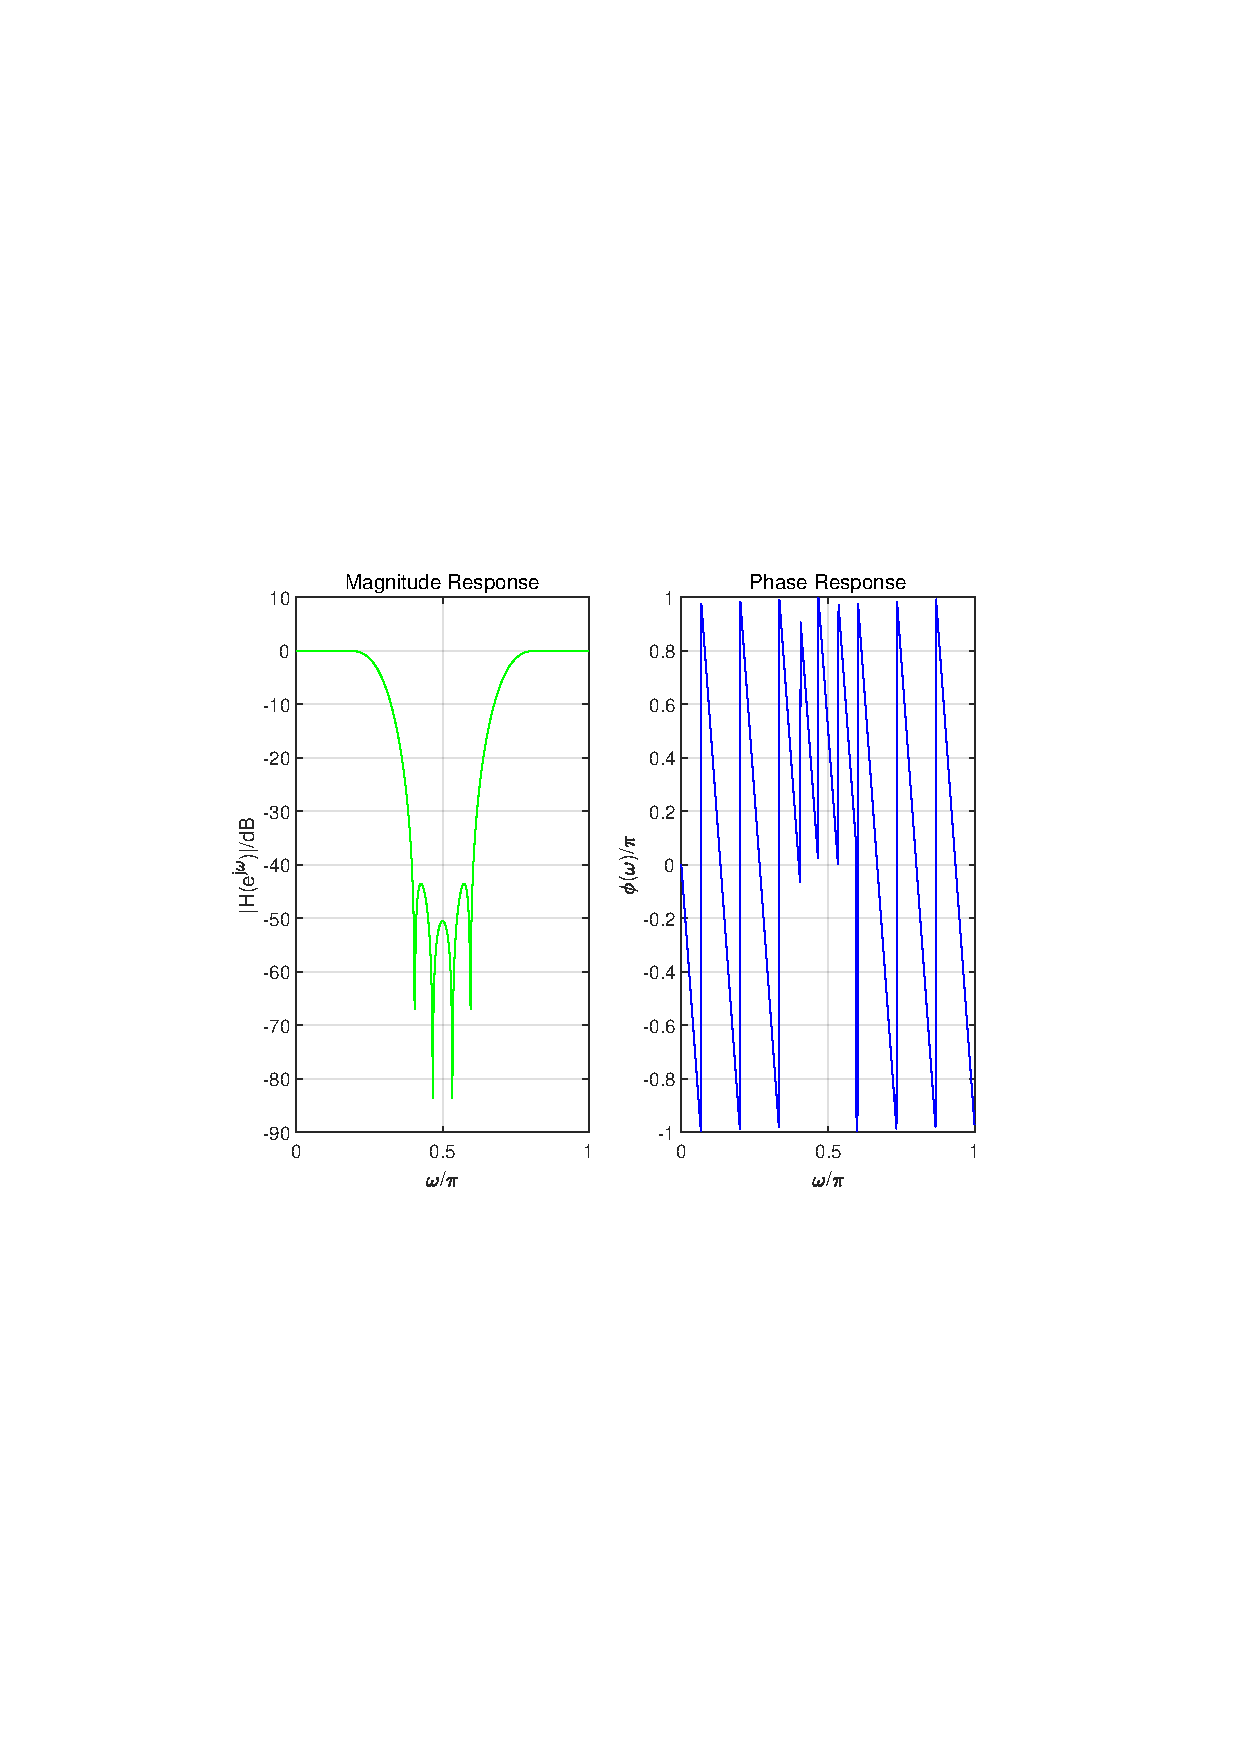
\includegraphics[width=0.7\textwidth]{figure/BS2.pdf}
	\caption{FIR 数字带阻滤波器单位频率响应曲线} \label{fig:BS2}
\end{figure}

\subsection{FIR 数字滤波器的结构信号流图}

\subsubsection{直接型}

FIR 数字滤波器的系统函数和差分方程分别为
%
\begin{equation}
H(z)=\sum_{n=0}^{N-1}h(n)z^{-n}
\end{equation}
%
和
\begin{equation}
y(n)=\sum_{m=0}^{N-1}h(m)x(n-m)
\end{equation}
%
直接由差分方程可画出 FIR 数字滤波器的直接型结构如图 \ref{fig:direct} 所示。

\begin{figure}[htbp]
	\centering
	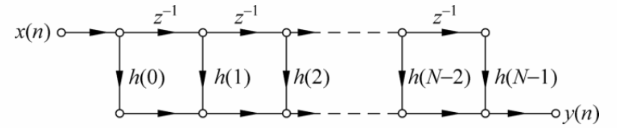
\includegraphics[width=0.7\textwidth]{figure/direct.png}
	\caption{FIR 数字滤波器的直接型结构} \label{fig:direct}
\end{figure}

\subsubsection{级联型}

当需要控制滤波器的传输零点时,可将系统函数分解为二阶实系数因子的形式:
%
\begin{equation}
H(z)= \sum_{n=0}^{N-1}h(n)z^{-n} =\prod_{i=1}^{M} \left(a_{0i}+a_{1i}z^{-1}+a_{2i}z^{-2}\right)
\end{equation}
%
于是可用二阶节级联构成,每一个二阶节控制一对零点,画出 FIR 数字滤波器的级联型结构如图 \ref{fig:cascade} 所示。

\begin{figure}[hbtp]
	\centering
	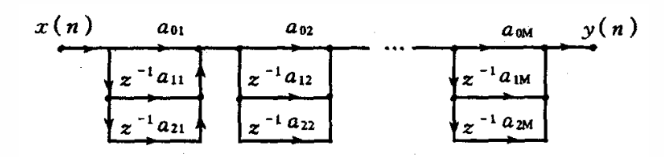
\includegraphics[width=0.7\textwidth]{figure/cascade.png}
	\caption{FIR 数字滤波器的级联型结构} \label{fig:cascade}
\end{figure}

\subsubsection{线性相位型}

线性相位是指滤波器产生的相移与输入信号频率成线性关系。如果 FIR 数字滤波器具有线性相位特性,它的单位脉冲响应满足下式:
%
\begin{equation}
h(n)=\pm h(N-n-1)
\end{equation}
%
其中:$h(n)$ 偶对称时,为第一类线性相位;$h(n)$ 及对称时,为第二类线性相位。

\begin{figure}[hbtp]
	\centering
	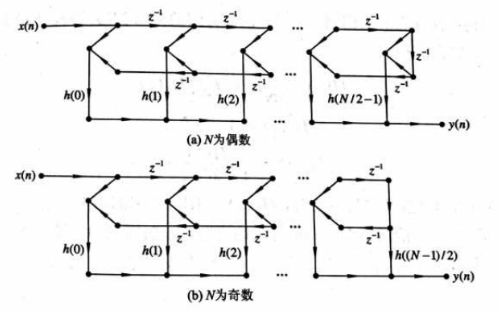
\includegraphics[width=0.7\textwidth]{figure/linear_phase1.png}
	\caption{FIR 数字滤波器的第一类线性相位型结构} \label{fig:linear_phase1}
\end{figure}

当 $N$ 为偶数时
%
\begin{equation}
H(z)=\sum_{n=0}^{N-1}h(n)z^{-n}=\sum_{n=0}^{\frac{N}{2}-1}h(n)\left[z^{-n}\pm z^{-(N-n-1)}\right]
\end{equation}
%
当 $N$ 为奇数时
%
\begin{equation}
H(z)=\sum_{n=0}^{N-1}h(n)z^{-n}=\sum_{n=0}^{\frac{N}{2}-1}h(n)\left[z^{-n}\pm z^{-(N-n-1)}\right]+h\left(\frac{N-1}{2}\right)z^{-\frac{N-1}{2}}
\end{equation}
%
由此可画出 FIR 数字滤波器的第一类和第二类线性相位型结构分别如图 \ref{fig:linear_phase1} 和图 \ref{fig:linear_phase2} 所示。

\begin{figure}[hbtp]
	\centering
	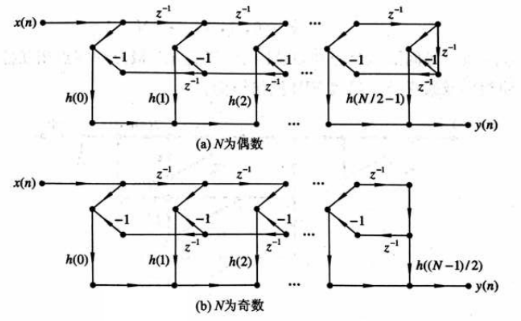
\includegraphics[width=0.7\textwidth]{figure/linear_phase2.png}
	\caption{FIR 数字滤波器的第二类线性相位型结构} \label{fig:linear_phase2}
\end{figure}

\subsubsection{频率采样型}

对系统函数取样可得:
%
\begin{equation}
H(k)=H(z)|_{z=e^{j\frac{2\pi}{N}k}}
\end{equation}
%
系统函数可由采样值 $H(k)$ 通过内插公式来表示,即
%
\begin{equation}
H(z)=\frac{1-z^{-N}}{N}\sum_{k=0}^{N-1}\frac{H(k)}{1-W_N^{-k}z^{-1}}
\end{equation}
%
可改写成:
%
\begin{equation}
H(z)=\frac{1}{N}H_c(z)\sum_{k=0}^{N-1}H_k(z)
\end{equation}
%
式中
%
\begin{align}
H_c(z) &= 1-z^{-N} \\
H_k(z) &= \frac{H(k)}{1-W_N^{-k}z^{-1}}
\end{align}
%

$H_c(z)$ 是一个梳状滤波器,它的零点在 $z_k=W_N^{-k}(0\le k\le N-1)$ 处;$H_k(z)$ 是一个一阶子系统,极点在 $p_k=W_N^{-k}(0\le k\le N-1)$ 处。FIR 数字滤波器的频率采样结构由一个 $N$ 阶梳状滤波器与 $N$ 个一阶子系统的并联网络级联而成,如图 \ref{fig:freq_sample} 所示。

\begin{figure}[hbtp]
	\centering
	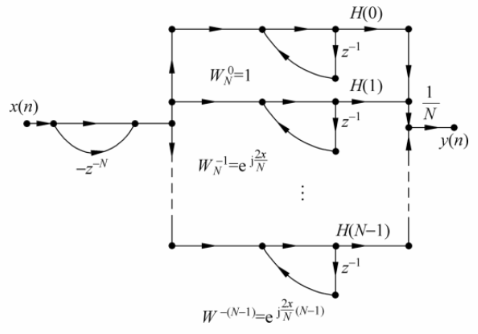
\includegraphics[width=0.7\textwidth]{figure/freq_sample.png}
	\caption{FIR 数字滤波器的频率采样型结构} \label{fig:freq_sample}
\end{figure}

\section{总结}

\subsection{杨文韬}

\begin{itemize}
\item 问题 1:相比 IIR 数字滤波器,FIR 数字滤波器有什么优势?
\begin{itemize}
\item 不需要反馈,因此舍去误差不会因为连续的加总而累计。每一次的计算其相对误差都是一样的,因此在实现上比较简单。
\item 在本质上稳定,因为其输出是有限个输入值乘以有限倍数的和。
\item 若让系数对称,可以设计成线性相位,这在一些相位很重要的应用(例如资料通讯、地震学或分音器)中是很好的特性。
\end{itemize}

\item 问题 2:从实验结果可用看出哪些结论?

从结果来看,滤波类型的不同,更多表现在频域上的不同,而在时域上不易看出什么不同。窗函数的长度主要影响的是滤波器的过渡带宽度。窗函数的长度 $N$ 越大,对应的主瓣宽度越窄,所以相应的滤波器的过渡带宽度越窄。

\item 问题 3:Python 中是否有类似的利用窗函数设计 FIR 数字滤波器函数?

scipy.signal 库中有类似函数,\lstinline[language=Python]|scipy.signal.firwin(numtaps, cutoff, width=None, window='hamming', pass_zero=True, scale=True, nyq=None, fs=None)|。numtaps 指滤波器的长度;cutoff 指滤波器的截止频率或一组截止频率;可选参数 width 若不为 None,则假定它是过渡区域的近似宽度 (用与 fs 相同的单位表示),用于Kaiser FIR滤波器设计;window 指希望使用的窗口。
\end{itemize}

\subsection{刘浩}

\begin{itemize}
\item 问题:FIR 数字滤波器信号流图各有什么特点?

\begin{itemize}
\item \textbf{直接型}:简单直观,乘法运算量较少,但调整零点较难。
\item \textbf{级联型}:调整零点比直接型方便。但 $H(z)$ 中的系数比直接型多,因而需要的乘法器多。当 $H(z)$ 的阶次高时,也不易分解。
\item \textbf{线性相位型}:在本质上是直接型,但乘法次数比直接型省了一半。
\item \textbf{频率采样型}:系数 $H(k)$ 直接就是滤波器在 $\omega=\frac{2\pi}{N}k$ 处的响应,因此,控制滤波器响应很直接。但所有系数 $W_N^{-k}$ 和 $H(k)$ 都是复数,计算复杂。有些极点实际上不能与梳状滤波器的零点相抵消,使系统的稳定性变差。
\end{itemize}
\end{itemize}

\subsection{周泽熙}

\begin{itemize}
\item 问题:在使用相关函数如何正确理解参数?

\lstinline[language=Matlab]|h=fir1(N-1,Wc,'ftype',window)|,其中 Wc 是关于 $\pi$ 的归一化的 6dB 数字截止频率,所以 Wc 在区间 $(0,1)$ 内。同时应注意 ftpye=high,设计高通滤波器,ftype=stop,设计带阻滤波器。当 window 缺省时,采用汉明窗;添加 bartlett(N) 改为三角窗;blackman(N) 布莱克曼窗;hanning(N) 汉宁;kaiser(N+1,beta),$\beta$=beta 的凯赛窗
\end{itemize}

% % 参考文献,此处以 MLA 引用格式为例

%\begin{thebibliography}{9}
%\end{thebibliography}

% % \includepdf[pages={1,2}]{Memo.pdf} 

% 可以直接导入pdf页面
\newpage
\begin{appendices}  % 附录环境
\section{实验代码}

\subsection{FIR 数字低通滤波器}

\begin{lstlisting}[language=Matlab]
% Low-pass filter
Wp=0.2*pi; Ws=pi/2; Rs=40; B=Ws-Wp;
beta=0.5842*(Rs-21)^0.4+0.07886*(Rs-21)
N0=ceil((Rs-7.95)/2.285/B)+1;
N=N0+mod(N0+1,2)
Wc=(Wp+Ws)/2/pi

h=fir1(N-1,Wc,kaiser(N,beta));

figure(1)
n=0:1:N-1;
stem(n, h, 'filled', 'MarkerSize', 3);
xlabel('n'); ylabel('h(n)');
title('Unit impulse response');

[H,W] = freqz(h,1,512);
figure(2)
subplot(1,2,1);
plot(W/pi,20*log10(abs(H)),'g'); grid on;
xlabel('\omega/\pi'); ylabel('|H(e^j^\omega)|/dB');
title('Magnitude Response');
subplot(1,2,2);
plot(W/pi,angle(H)/pi,'b');grid on;
xlabel('\omega/\pi'); ylabel('\phi(\omega)/\pi');
title('Phase Response');
\end{lstlisting}

\subsection{FIR 数字高通滤波器}

\begin{lstlisting}[language=Matlab]
% High-pass filter
Wp=pi/2; Ws=0.2*pi; B=Wp-Ws;
N0=ceil(6.2*pi/B);
N=N0+mod(N0+1,2)
Wc=(Wp+Ws)/2/pi

h=fir1(N-1,Wc,'high',hanning(N));

figure(1)
n=0:1:N-1;
stem(n, h, 'filled', 'MarkerSize', 3);
xlabel('n'); ylabel('h(n)');
title('Unit impulse response');

[H,W] = freqz(h,1,512);
figure(2)
subplot(1,2,1);
plot(W/pi,20*log10(abs(H)),'g');grid on;
xlabel('\omega/\pi'); ylabel('|H(e^j^\omega)|/dB');
title('Magnitude Response');
subplot(1,2,2);
plot(W/pi,angle(H)/pi,'b');grid on;
xlabel('\omega/\pi'); ylabel('\phi(\omega)/\pi');
title('Phase Response');
\end{lstlisting}

\subsection{FIR 数字带通滤波器}

\begin{lstlisting}[language=Matlab]
% Band-pass filter
Wp1=0.4*pi; Ws1=0.2*pi;
Wp2=0.6*pi; Ws2=0.8*pi;
B=Wp1-Ws1;
N0=ceil(6.2*pi/B);
N=N0+mod(N0+1,2)
Wc=[(Wp1+Ws1)/2/pi,(Wp2+Ws2)/2/pi]

h=fir1(N-1,Wc,hanning(N));

figure(1)
n=0:1:N-1;
stem(n, h, 'filled', 'MarkerSize', 3);
xlabel('n'); ylabel('h(n)');
title('Unit impulse response');

[H,W] = freqz(h,1,512);
figure(2)
subplot(1,2,1);
plot(W/pi,20*log10(abs(H)),'g');grid on;
xlabel('\omega/\pi'); ylabel('|H(e^j^\omega)|/dB');
title('Magnitude Response');
subplot(1,2,2);
plot(W/pi,angle(H)/pi,'b');grid on;
xlabel('\omega/\pi'); ylabel('\phi(\omega)/\pi');
title('Phase Response');
\end{lstlisting}

\subsection{FIR 数字带阻滤波器}

\begin{lstlisting}[language=Matlab]
% Band-stop filter
Wp1=0.2*pi; Ws1=0.4*pi;
Wp2=0.8*pi; Ws2=0.6*pi;
B=Ws1-Wp1;
N0=ceil(6.2*pi/B);
N=N0+mod(N0+1,2)
Wc=[(Wp1+Ws1)/2/pi,(Wp2+Ws2)/2/pi]

h=fir1(N-1,Wc,'stop',hanning(N));

figure(1)
n=0:1:N-1;
stem(n, h, 'filled', 'MarkerSize', 3);
xlabel('n'); ylabel('h(n)');
title('Unit impulse response');

[H,W] = freqz(h,1,512);
figure(2)
subplot(1,2,1);
plot(W/pi,20*log10(abs(H)),'g');grid on;
xlabel('\omega/\pi'); ylabel('|H(e^j^\omega)|/dB');
title('Magnitude Response');
subplot(1,2,2);
plot(W/pi,angle(H)/pi,'b');grid on;
xlabel('\omega/\pi'); ylabel('\phi(\omega)/\pi');
title('Phase Response');
\end{lstlisting}

%\section{核心层}\label{subsec:B}
\end{appendices}

\end{document}  % 结束